 %%%%%%%%%%%%%%%%%%%%%%%%%%%%%%%%%%%%%%%%%%%%%%%%%%%%%%%%%%%%%%%%%%%%%%%%%%%%%%%%%%
%%																				%%
%% File name: 		01sarah.tex													%%
%% Project name:	Hochleistungsantenne										%%
%% Type of work:	T3X00 project work											%%
%% Author:		Sarah Brückner, Maximilian Stiefel, Hannes Bohnengel		%%
%% Date:		27th Arpil 2016												%%
%% University:		DHBW Ravensburg Campus Friedrichshafen						%%
%% Comments:		Created in gedit with tab width = 4							%%
%%																				%%
%%%%%%%%%%%%%%%%%%%%%%%%%%%%%%%%%%%%%%%%%%%%%%%%%%%%%%%%%%%%%%%%%%%%%%%%%%%%%%%%%%

\chapter{Amateurfunksatelliten}
In dieser Studienarbeit soll die Bodenstation erdnahe Satelliten verfolgen können. Erdnah bedeutet auf einer niedrigen Umflaufbahn bis etwa 1200 km. 
Dazu gehören die Amateurfunksatelliten, welche der Satellitenkommunikation zwischen Funkamateuren und auch zu experimentellen Zwecken dienen. 
Diese kommunizieren im 2-Meter- und 70-Zentimeterband \cite{Wiki:amateur} und ermöglichen einen internationalen Sprech- und Datenfunk. Außerdem senden diese Satelliten
auch Messwerte der Betriebsdaten des Satelliten. Diese Satelliten werden meist von Hochschulen oder Amateurfunkvereinigungen gebaut und mit weiteren 
Satelliten an Board einer Rakete in das All geschossen. Dabei handelt es sich um kleine, leichte Satelliten, auch ``Cubesat'' genannt.
\begin{figure}[h]
 \centering
 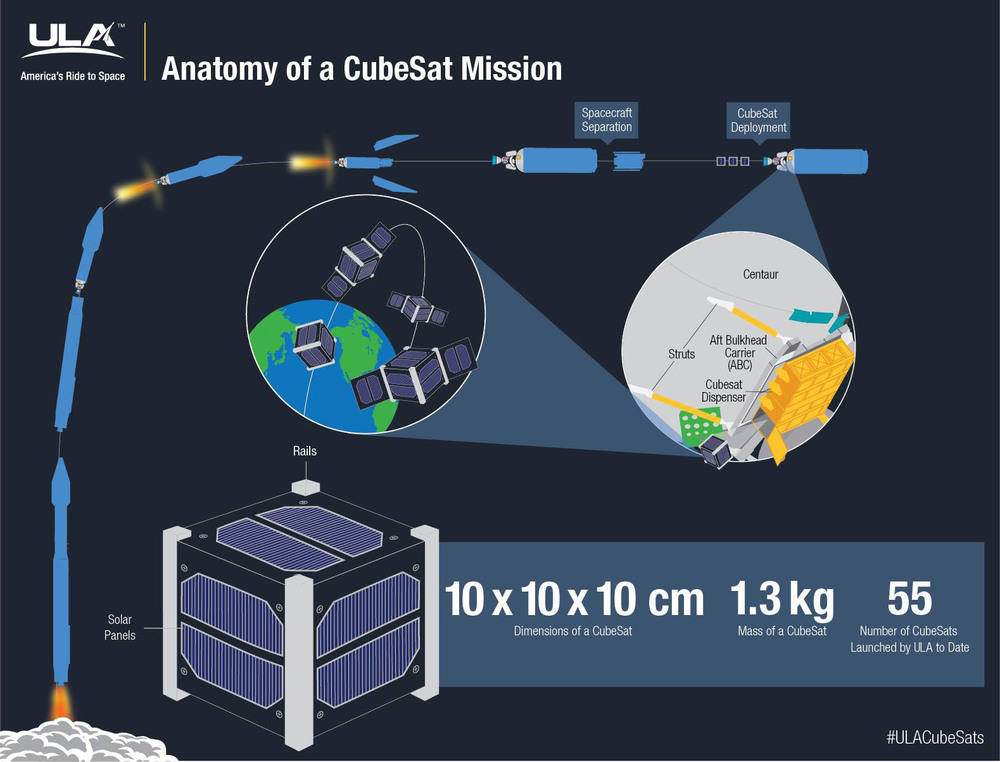
\includegraphics[width=0.8\linewidth]{./images/cubesat}
 \caption{Cubesat, Quelle: \cite{cubesat}}
 \label{fig:cubesat}
\end{figure}
Die Grafik \ref{fig:cubesat} zeigt einen beispielhaften Cubesat und wie dieser von einer Rakte in das All geschossen wird. Im Vergleich, der ASTRA 1L Satellit mit 
einer Spannweite von 20 Meter und einem Gewicht von 4,5 Tonnen. Erdnahe Satelliten umkreisen die Erde städnig und haben daher nur ein beschränktes 
Zeitfenster, in dem man mit einem solchen Satelliten arbeiten kann. Davor befindet sich der Satellit durch die Erdkrümmung hinter dem Horizont und 
ist daher unerreichbar. Daher ist es für die Bodenstation wichtig zu wissen wann der Satellit am Horizont auftaucht um die Antenne in die richtige 
Position nachzuführen. Nach der korrekten Nachführung folgt die Kontaktaufnahme. Die Amateurfunksatelliten arbeiten in einem bestimmten Modus. 
Der Modus gibt an, in welchem Frequenzbereich der Satellit hört und auf welchem er sendet. Ein Signal,
das der Satellit zur Erde schickt nennt man ``Downlink'' und von der Basisstation zum Satelliten ``Uplink''. Das für diese Studienarbeit 
verwendete Funkgerät IC-9100 kann mit den Modis B und J arbeiten \cite[S.153]{radiomanual}
\begin{itemize}
 \item Mode B: Uplink: 70 cm - Downlink:  2  m 
 \item Mode J: Uplink:  2  m - Downlink: 70 cm
\end{itemize}
Einige Cubesats senden in \ac{CW} das Rufzeichen sowie ihre Telemetriedaten aus und dient der Funktionskontrolle.
\newpar
